\documentclass[amsfonts, amssymb, aps, nofootinbib, twocolumn]{revtex4-2}
\usepackage[T1]{fontenc}
\usepackage{tgtermes}
\usepackage{amsmath}
\usepackage{empheq}
\usepackage{enumitem}
\usepackage{graphicx}
\usepackage{booktabs}
\usepackage[braket, qm]{qcircuit}
\usepackage{braket}
\usepackage{hyperref}
\usepackage{xcolor}
\usepackage{tikz}
\hypersetup{
	colorlinks   = true, %Colours links instead of ugly boxes
	urlcolor     = blue, %Colour for external hyperlinks
	linkcolor    = blue, %Colour of internal links
	citecolor   = red %Colour of citations
}

\newcommand{\CZ}{CZ }
\newcommand{\CX}{CNOT }
\newcommand{\CP}{CP }
\newcommand{\T}{T }
\newcommand{\tgate}[1]{\textcolor{blue}{#1}}
\newcommand{\cx}[1]{C${}^{#1}$X}
\newcommand{\cz}[1]{C${}^{#1}$Z}
\newcommand{\package}[1]{\textrm {#1 }}
\newcommand{\cpflow}{\package{CPFlow}}
\newcommand{\static}{\textsc{static }}
\newcommand{\adaptive}{\textsc{adaptive }}
\newcommand{\param}[1]{\texttt{#1}}
\begin{document}
\title{Variational synthesis of quantum circuits by coherent architecture optimization}
\begin{abstract}
We consider the problem of the variational quantum circuit synthesis into a gate set consisting of the \CX gate and arbitrary 1q gates with the primary target being the minimization of the \CX count. First we note that along with the discrete architecture search, a clear combinatorial challenge, optimization over 1q gates can also be a crucial roadblock due to the omnipresence of local minimums (well known in the context of variational quantum algorithms but apparently underappreciated in the context of variational compiling). Taking the issue seriously we make extensive search over the initial conditions an essential part of our approach. 

Another key idea we propose is to use parametrized 2q \CP gates, which can interpolate between the identity gate and the \CX gate, and allow to reformulate the discrete architecture search as a continuous optimization problem, which can be executed jointly with the optimization over 1q gates. This coherent optimization of the architecture together with 1q gates appears to work surprisingly well in practice, sometimes even outperforming optimization over 1q gates alone (for a fixed optimal architecture).

As applications we derive 8 \CX and \T depth 3 decomposition of the 3q Toffoli gate on the nearest-neighbor topology, rediscover known best decompositions of the 4q Toffoli gate on all 4q topologies including a  1 \CX gate improvement on the star-shaped topology, and propose decomposition of the 5q Toffoli gate on the nearest neighbor topology with 48 \CX gates. We also benchmark performance of our approach on a number of 5q quantum circuits from the ibm\_qx\_mapping database showing that in many cases it reliably outperforms existing software. The algorithm developed in this work is available as a Python package \cpflow \cite{}. 
\end{abstract}
\maketitle	
\tableofcontents
\section{Introduction}
While many quantum algorithms such prime factoring \cite{Shor1997}, unstructured search \cite{Grover1997} or linear equation solver \cite{Harrow2009} promise game-changing speed ups over classical, the current state of the technology does not yet allow for a decisive demonstration with useful applications, although it might be on the verge (see e.g. here for a recent review \cite{Fedorov2022}). There are plenty of factors limiting performance of the current quantum devices, such as initialization and readout errors, loss of coherence over time and errors in gate operations. In the current NISQ era \cite{Preskill2018} most gate-based quantum protocols are constructed out of 1q and 2q gates with the latter being significantly more error-prone across all leading platforms. Hence, minimization of the 2q gate count is one of the key objectives that can improve performance of the near-term algorithms. On the other hand, in the fault-tolerant future a different type of resource (e.g. the \T gate count) is likely to be the most expensive.

At the high level quantum algorithms are usually described using primitives such as large multi-controlled gates or quantum Fourier transform that aren't directly accessible on the current devices. The usual compiling routines \cite{Qiskit, Sivarajah2021} include decomposing algorithmic primitives into native gates (which is always possible \cite{Barenco1995}), routing stage to comply with the possible connectivity restrictions of the target chip, and local simplifications of the resulting circuits. Using special datastructures for representing and transforming circuits allows to carry out the compilation process without the need to simulate any part of the circuit. This makes the approach extremely scalable, allowing to compile and optimize circuits with hundreds of qubits. The downside is that the resulting decompositions may be significantly less efficient than possible. A complementary approach is to work directly with the unitary matrix of the circuit thus eliminating any potential redundancies or inefficiencies in the original gate-based description. This is only feasible for small scale circuits as the size of the state space and the corresponding unitary matrices scales exponentially (even for a small number of qubits there may be other limiting factors such as circuit complexity, as we emphasize in this work). Although there could be direct applications to enhancing performance of the NISQ algorithms, we expect that the use highly optimized small scale circuits as building blocks of large scale algorithms to be the most promising possibility.

The unitary synthesis problem amounts to finding the most efficient circuits optimizing a given loss function. Typical applications include minimizing fidelity with respect to the target unitary (compilation) or maximizing the overlap with the target state (state preparation). We consider the problem of the variational synthesis into the gate set consisting of a single 2q gate (\CZ or \CX) and arbitrary 1q gates. The primary optimization target is the amount of \CX gates, although indirectly we also address \CX depth and even \T count and \T depth. It is natural to divide the problem into two parts:
\begin{enumerate}[label=(\roman*), nosep]
	\item Discrete optimization or architecture search, looking for best placements of 2q gates.
	\item Continuous optimization of 1q gate parameters for a given architecture.
\end{enumerate}
The difficulty associated with the architecture search has combinatorial origin and is manifest. The difficulty of the continuous optimization is however also essential, as is known in the context of variational quantum algorithms, but apparently underappreciated in the context of variational compiling. We zoom in on this issue in section sec.\ref{sec local minimums}. Another cornerstone idea of our approach is to use parametrized 2q gates as a means to reduce discrete architecture search to another continuous optimization that can be performed simultaneously and coherently with learning the angles 1q gates. We introduce the \cpflow algorithm in sec.\ref{sec cpflow}. In sec.\ref{sec toffoli} we first illustrate all central features of the \cpflow on the example of the 3q Toffoli gate and then go beyond this toy example to synthesize efficient (and likely novel) decompositions on constrained topologies in the 4q and 5q case. In sec.\ref{sec benchmark} we provide further benchmarks showcasing that \cpflow is very efficient in compilation of small scale circuits with moderate complexity but also outline its limitations. Sec.\ref{sec last} concludes with the summary and outlook.

\textbf{\textit{Related work}}. The idea to use computer assisted search and numerical optimization for circuit synthesis goes back a long way \cite{Divincenzo1994} and continues to the present day with advances due to both algorithm design and growth of raw computational power. Possible frameworks include purely discrete search over a finite gate set \cite{Nagarajan2021}, a natural separation into discrete architecture search and continuous optimization \cite{Nam2018, Khatri2019, Smith2021} and a hybrid approach with part of the architecture search outsourced to a version of continuous optimization \cite{Younis2021, Rakyta2022}. The scheme developed in \cite{Rakyta2022} is in many respects similar to the one proposed in this paper, and similarly to our work, was originally motivated by the impressive success of variational compiling of random unitaries (maximum complexity circuits) \cite{Kiani2020, Madden2021, Rakyta2021}. 

\section{Background and notation}
\subsection{Template circuits}
The prevalent approach in the literature \cite{Khatri2019, Madden2021, Rakyta2021, Nakanishi2021, Rakyta2022} that we will follow is to construct the template circuits out of two-qubit blocks repeated in a regular manner. The two types of entangling blocks we will use are CZ- and CP-blocks depicted at fig.\ref{fig blocks}. They only differ by the type of the entangling gates used. We will explain the choice of 1q gates shortly.
\begin{figure}
\begin{flushleft}
(a)
\scalebox{1.0}{
	\Qcircuit @C=1.0em @R=0.2em @!R { \\
		& \ctrl{1} & \gate{\mathrm{R_X}\,(\mathrm{a_0})} & \gate{\mathrm{R_Y}\,(\mathrm{a_2})} & \gate{\mathrm{R_Z}\,(\mathrm{a_4})} & \qw & \qw\\
		& \control\qw & \gate{\mathrm{R_X}\,(\mathrm{a_1})} & \gate{\mathrm{R_Y}\,(\mathrm{a_3})} & \gate{\mathrm{R_Z}\,(\mathrm{a_5})} & \qw & \qw\\
		\\ }}\\
(b)
	\scalebox{1.0}{
	\Qcircuit @C=1.0em @R=0.2em @!R { \\
		& \ctrl{1} & \dstick{\hspace{2.0em}\mathrm{P}\,(\mathrm{a_5})} \qw & \qw & \qw & \gate{\mathrm{R_X}\,(\mathrm{a_0})} & \gate{\mathrm{R_Y}\,(\mathrm{a_2})} & \gate{\mathrm{R_Z}\,(\mathrm{a_4})} & \qw & \qw\\
		& \control \qw & \qw & \qw & \qw & \gate{\mathrm{R_X}\,(\mathrm{a_1})} & \gate{\mathrm{R_Y}\,(\mathrm{a_3})} & \gate{\mathrm{R_Z}\,(\mathrm{a_5})} & \qw & \qw\\
		\\ }}
\end{flushleft}
\caption{(a) CZ block (b) CP block.}
\label{fig blocks}
\end{figure}
The blocks are further arranged in sequences we refer to as \textit{layers}. In principle, layers can can be arbitrary, but we will usually identify layers with coupling maps of the target topology. For example see fig.\ref{fig layers} showing layers corresponding the fully connected and chain (or nearest-neighbor) topology.
\begin{figure}
(a)	Connected layer \qquad\qquad(b) Chain layer
\\
\scalebox{1.0}{
	\Qcircuit @C=1.0em @R=0.8em @!R { \\
		 & \ctrl{1} & \ctrl{2} & \ctrl{3} & \qw & \qw & \qw & \qw \\
		& \control\qw & \qw & \qw & \ctrl{1} & \ctrl{2} & \qw & \qw \\
		& \qw & \control\qw & \qw & \control\qw & \qw & \ctrl{1} & \qw\\
		& \qw & \qw & \control\qw & \qw & \control\qw & \control\qw & \qw \\
		\\ }}\qquad\qquad
\scalebox{1.0}{
	\Qcircuit @C=1.0em @R=0.8em @!R { \\
		& \ctrl{1} & \qw & \qw & \qw\\
		& \control\qw & \ctrl{1} & \qw & \qw\\
		& \qw & \control\qw & \ctrl{1} & \qw\\
		& \qw & \qw & \control\qw & \qw\\
		\\ }}
\caption{(a) 4q connected layer (b) 4q chain layer. Here CZ gates are only meant to specify locations of 2q blocks, not their content. }
\label{fig layers}
\end{figure}

Finally, to fully specify the template one must provide the total \textit{number of 2q gates}. Layers are repeated until the specified number of 2q gates is reached, the last layer is truncated if needed. We will write $U^k_{CZ}$ or $U^k_{CP}$ for templates with $k$ entangling gates of type \CZ or \CP respectively (layer specification is assumed but left implicit in the notation). For illustration, fig.\ref{fig template example} depicts $U^4_{CZ}$ on a connected topology.

\begin{figure*}
\scalebox{0.65}{
	\Qcircuit @C=1.0em @R=0.2em @!R {
		&&&&&&&&&&&&&&&&&&&&&&&\\
		& \gate{\mathrm{Z}\,(\mathrm{a_{0}})} & \gate{\mathrm{X}\,(\mathrm{a_{1}})} & \gate{\mathrm{Z}\,(\mathrm{a_{2}})} & \ctrl{1} & \gate{\mathrm{X}\,(\mathrm{a_{9}})} & \gate{\mathrm{Y}\,(\mathrm{a_{11}})} & \gate{\mathrm{Z}\,(\mathrm{a_{13}})} & \ctrl{2} & \gate{\mathrm{X}\,(\mathrm{a_{15}})} & \gate{\mathrm{Y}\,(\mathrm{a_{17}})} & \gate{\mathrm{Z}\,(\mathrm{a_{19}})} & \qw & \qw & \qw & \qw & \qw & \qw &\ctrl{1} & \gate{\mathrm{X}\,(\mathrm{a_{27}})} & \gate{\mathrm{Y}\,(\mathrm{a_{29}})} & \gate{\mathrm{Z}\,(\mathrm{a_{31}})} & \qw & \qw\\
		& \gate{\mathrm{Z}\,(\mathrm{a_{3}})} & \gate{\mathrm{X}\,(\mathrm{a_{4}})} & \gate{\mathrm{Z}\,(\mathrm{a_{5}})} & \control\qw & \gate{\mathrm{X}\,(\mathrm{a_{10}})} & \gate{\mathrm{Y}\,(\mathrm{a_{12}})} & \gate{\mathrm{Z}\,(\mathrm{a_{14}})} & \qw & \qw & \qw & \qw & \ctrl{1} & \gate{\mathrm{X}\,(\mathrm{a_{21}})} & \gate{\mathrm{Y}\,(\mathrm{a_{23}})} & \gate{\mathrm{Z}\,(\mathrm{a_{25}})} & \qw & \qw & \control\qw & \gate{\mathrm{X}\,(\mathrm{a_{28}})} & \gate{\mathrm{Y}\,(\mathrm{a_{30}})} & \gate{\mathrm{Z}\,(\mathrm{a_{32}})} & \qw & \qw\\
		& \gate{\mathrm{Z}\,(\mathrm{a_{6}})} & \gate{\mathrm{X}\,(\mathrm{a_{7}})} & \gate{\mathrm{Z}\,(\mathrm{a_{8}})} & \qw & \qw & \qw & \qw & \control\qw & \gate{\mathrm{X}\,(\mathrm{a_{16}})} & \gate{\mathrm{Y}\,(\mathrm{a_{18}})} & \gate{\mathrm{Z}\,(\mathrm{a_{20}})} & \control\qw & \gate{\mathrm{X}\,(\mathrm{a_{22}})} & \gate{\mathrm{Y}\,(\mathrm{a_{24}})} & \gate{\mathrm{Z}\,(\mathrm{a_{26}})} & \qw & \qw & \qw & \qw & \qw & \qw & \qw & \qw
		\gategroup{1}{5}{5}{17}{1.em}{-}
		\gategroup{1}{19}{5}{23}{1.em}{--}\\
		&&&&&&&&&&&&&&&&&&&&&&&
}}	
\caption{Template circuit $U^4_{CZ}$ on a connected 3q topology with 4 entangling \CZ-blocks. The complete connected layer is boxed, the incomplete layer is dash-boxed.}
\label{fig template example}
\end{figure*}

\subsection{Theoretical lower bound \ref{sec tlb}}
There is a provable minimum amount of \CZ gates required to decompose any $n$-qubit unitary \cite{Shende2004} that we will refer to as the \textit{theoretical lower bound}
\begin{align}
TLB(n) = \frac14\left(4^n-3n-1\right) \ . \label{TLB}
\end{align}
It essentially follows from the simple parameter counting argument. We will sketch the argument which is not only instructive but also helps us to motive the ansatz structure for the template circuits. A unitary matrix on $n$ qubits has in general $4^n$ real parameters. An arbitrary 1q gate on the other hand has 3 real parameters, e.g. angles in the Euler decomposition. Thus, without 2q gates a quantum circuit with $n$ qubits can have no more that $3n$ real parameters. Our template circuits start with a round of 1q gate, cf fig.\eqref{fig template example}. Now, adding a single \CZ gate allows to add two more single qubits gates that do not combine with the existing ones. However, one parameter in each of the single qubit blocks is redundant as illustrated at fig.\ref{fig ZXZ}. Using ZXZ decomposition of an arbitrary single-qubit block $U$ and the fact that $R_Z$ commutes with the the \CZ-gate the leftmost $R_Z$ blocks on each qubit can be pulled to the left and joined with the existing 1q blocks. Therefore adding a single entangling \CZ-block allows to add four more real parameters to the circuit. Requiring that $4TLB(n)+3n=4^{n}-1$ leads to \eqref{TLB} (additional unit subtracted is the irrelevant global phase parameter).

\begin{figure}
\begin{align*}
\scalebox{0.85}{
\Qcircuit @C=0.5em @R=0.4em @!R {
	& \ctrl{1} & \gate{\mathrm{U}} & \qw & \qw\\
	& \control\qw & \gate{\mathrm{U}} & \qw & \qw\\
} 
\quad\raisebox{-1.em}{=}\quad
\Qcircuit @C=0.5em @R=0.4em @!R {	
	& \ctrl{1} & \gate{R_Z} & \qw& \gate{R_X} & \qw& \gate{R_Z} & \qw  & \qw\\
	& \control\qw & \gate{R_Z} & \qw& \gate{R_X} & \qw& \gate{R_Z} & \qw & \qw\\
}
\quad\raisebox{-1.em}{=}\quad
\Qcircuit @C=0.5em @R=0.4em @!R {	
	& \gate{R_Z} & \qw& \ctrl{1} & \gate{R_X} & \qw& \gate{R_Z} & \qw  & \qw\\
	& \gate{R_Z} & \qw& \control\qw & \gate{R_X} & \qw& \gate{R_Z} & \qw & \qw \\
}}
\end{align*}
\caption{Entangling \CZ-block only allows to add four real parameters to the circuit. Explicit gate angles are not depicted.}
\label{fig ZXZ}
\end{figure}

While \eqref{TLB} is a simple theoretical bound, there is strong evidence for its tightness. First of all, there is an constructive analytic procedure, known as the quantum Shannon decomposition \cite{Shende2006}, which produces decomposition of any given unitary using lying only a factor $\frac{23}{12}TLB(n)$ away from the theoretical lower bound. Second, recent studies involving numerical experiments \cite{Madden2021, Rakyta2021} imply that the $\approx2x$ overhead of the quantum Shannon decomposition is not necessary and that \CZ count given by \eqref{TLB} is sufficient to compile random unitaries with a great numerical accuracy.

So far our discussion and the bound \eqref{TLB} addressed generic or random unitaries. However, the unitary matrices of the central importance to quantum computation are highly structured and typically require much less 2q gates. The quantum Shannon decomposition does not appear to be particularly useful in this case. It's extension to not fully-connected topologies is also difficult, often leading to an large multiplicative overhead \cite{Shende2006}. Note that being able to find truly optimal decompositions would amount to determining the gate complexity of a unitary matrix which is an $NP$-complete problem \cite{Botea2018}.

It is therefore a natural idea to use numeric optimization and heuristic methods in the search of efficient decompositions. This strategy is known as the variational compiling and have been explored in a range of works \cite{}. In the next section we review the variational compiling and associated challenges.

\section{Variational synthesis and its challenges \label{sec local minimums}}

\begin{figure*}
	\includegraphics[width=0.4\textwidth]{figures/3q_success_chart}
	\includegraphics[width=0.4\textwidth]{figures/4q_success_chart}
	\caption{Local minimums as a function of circuit complexity. Datapoints for random unitaries are advanced by a half unit along $x$ axis for clarity.}
	\label{fig local minumums}
\end{figure*}

Decomposition into 2q and 1q gates implies that two problems need to be solved:
\begin{itemize}
	\item Discrete optimization problem or architecture search, concerned with finding optimal placements for 2q gates.
	\item Continuous optimization problem of finding suitable parameters of 1q gates for a given architecture.
\end{itemize}
While the difficulty of the architecture search has a combinatorial origin and hardly needs explaining, the difficulty of continuous optimization also can not be ignored. Mathematically the problem of variational synthesis is very similar to the classical optimization loop in quantum variational algorithms \cite{}, especially their hardware-efficient \cite{Kandala2017} and adaptive \cite{} forms . Here, the two key obstacles are the \textit{barren plateaus} and \textit{local minimums}. The barren plateaus manifest as vanishing gradients and are usually associated with large number of qubits or parameters. In our experiments with small-scale quantum circuits we did not find it to be relevant. On the other hand, the problem of local minimums alone is sufficient to render training of the variational algorithms $NP$-hard \cite{Bittel2021} in the worst case. As our numerical experiments suggest, local minimums constitute a real hindrance to the variational compiling.

We will quantify the challenges associated with local minimums by the empirical success ratio
\begin{align}
	SR=\frac{M}{N} \ ,
\end{align}
where $N$ is the total number of times the optimization procedure is performed starting with different random initial conditions and $M$ is the number of times a global minimum is reached. 

For example, let $U(a)$ be the unitary matrix of the template circuit from fig.\ref{fig template example} and $a^*$ be some particular choice of angles. It is clear that the global minimum of the Hilbert-Schmidt distance $D(U(a), U(a^*))$ is zero, but gradient-based optimization does not always reach it. With some particular random choice of $a^*$ and random uniform initialization of the template angles our default optimization (detailed in \ref{}) yields success ratio $SR\approx0.3$, which implies that roughly two third of the times the optimization gets stuck in a local minimum. 

We now extend this simple numerical experiment more systematically. Fig.\ref{fig local minumums} charts the success ratios for 3q and 4q circuits as a function of the number of gates. The basic procedure is the same with several additions. First, we used templates with fully connected layers (see fig.\ref{fig layers}) extended to the required number of 2q gates. For each number of 2q gates we take 10 different random parameter assignments $a^*$ and compute success ratios for each of them using 1000 initial conditions, generated uniformly at random. Blue markers represent mean success ratios averaged over 10 target circuits, while error bars quantify the mean standard deviation. Absence of blue markers implies that the empirical success ratio turned out vanishing, i.e. that the global minimum was not reached. For 4q circuits datapoints were only collected for every third gate count.

There are several remarkable features of the graph. First, the success ratio drops very quickly as the 2q gate count increases, reaching values below $10^{-3}$ at 10 \CZ gates for 3q circuits and 15 \CZ gates fro 4q circuits. Next, perhaps surprisingly, the success ratio rises back to values of order 1 as the number of \CZ gates approaches the theoretical lower bound \eqref{TLB}. In fact, this is in agreement with the empirical evidence found in the literature \cite{Madden2021, Rakyta2021, Kiani2020} that near the theoretical lower bound numerical compilation appears to be very efficient. A plausible explanation for this fact \cite{Ge2022} is that when the template is sufficiently expressive, optimization w.r.t. parameters becomes essentially the same as optimization over the unitary matrices themselves. At the same time, cost functions typically considered in quantum computing are simple, often linear or quadratic functions of the unitary matrix elements and hence are not prone to local minimums. Finally, although there is a certain spread of success ratios across different template instances, dependence on the 2q gate count sets the dominating trend.

This suggests that success ratio is mostly determined by the template, not by the target. To confirm this  intuition  we carried out additional experiments using random unitaries $V$ instead of template instances as targets. The difficulty here is that the true value of the global minimum of $D(U(a), V)$ is not known, but the presence of local minimums is still manifest. We modify definition of the success ratio in this case, by counting as successful all optimization runs that approached sufficiently closely the lowest value of $D$ across all runs for a given target unitary. Note that with this modified definition the success ratio can never be zero (because there is always at least a single run with the lowest value). We see that in the regime when success ratios for random instances are sufficiently high success ratios for random unitaries closely parallel them, both in mean and in deviation. In the regions where success ratios for random instances are very small or vanishing, success ratios for random unitaries are non-zero (they can not be by construction) but are sufficiently close to zero. We expect them to drop further if more samples are accounted for. Overall, our experiments strongly suggest that local minimums are mostly determined by the templates and not by targets.

Of course, success ratio is not only a function of the loss landscape but also of the optimization algorithm and the distribution of the initial conditions. There are a number of proposals to alleviate the problem of local minimums by the choice of optimizer \cite{Wierichs2020, Rivera-Dean2021}, but in our experiments none performed sufficiently better than simple ADAM\cite{adam}-based optimization to justify additional computational resources that are typically required by higher-order methods such as the natural gradient \cite{Stokes2020} or imaginary time evolution \cite{Jones2018a}. A recent empirical comparison of various optimization methods for quantum variational algorithms \cite{Lockwood2022} also suggests that the ADAM algorithm can be a simple and efficient choice.

In turn, our own experiments suggest that parametrization and/or distribution of the initial parameters can make a big difference. As explained in \ref{sec tlb} template structure illustrated at fig.\ref{fig template example} features redundant 1q gates. In any entangling block two rotation gates can be removed without compromising circuit expressivity, i.e. without any shrinking in the space of all unitaries obtainable from the template. However, performance of the templates with the minimal number of 1q gates appears to be worse on average (though there are counter examples, see sec.\ref{sec toff4}). This can be due to the fact that overparmetrization favorably deforms the loss landscape and/or because random uniform initialization of the angles produces a different distribution of the initial unitaries. In the present study we do not attempt to disentangle the two possible effects and leave this important question for future work. Unless stated otherwise, reported results correspond to the 'XYZ' templates as per fig.\ref{fig template example}.
\section{The CPFlow algorithm \label{sec cpflow}}
\subsection{Motivation and overview}
In the context of variational synthesis results of the previous section suggest that solving the continuous optimization problem may be just as difficult as solving the discrete architecture search: even if the structure of the template is a perfect match for the target unitary, finding the suitable angles may be very challenging. In the absence of an efficient way to solve the latter problem in our approach we choose the brute force route of trying many initial conditions. 
\begin{figure*}
	\scalebox{0.7}{
		\Qcircuit @C=1.0em @R=0.2em @!R { \\
			& \gate{\mathrm{Z}\,(\mathrm{a_{0}})} & \gate{\mathrm{X}\,(\mathrm{a_{1}})} & \gate{\mathrm{Z}\,(\mathrm{a_{2}})} & \ctrl{1} & \dstick{\hspace{2.0em}\mathrm{P}\,(\mathrm{a_{15}})} \qw & \qw & \qw & \gate{\mathrm{X}\,(\mathrm{a_{9}})} & \gate{\mathrm{Y}\,(\mathrm{a_{11}})} & \gate{\mathrm{Z}\,(\mathrm{a_{13}})} & \ctrl{2} & \qw & \qw & \qw & \gate{\mathrm{X}\,(\mathrm{a_{16}})} & \gate{\mathrm{Y}\,(\mathrm{a_{18}})} & \gate{\mathrm{Z}\,(\mathrm{a_{20}})} & \qw & \qw & \qw & \qw & \qw & \qw & \qw & \qw & \qw\\
			& \gate{\mathrm{Z}\,(\mathrm{a_{3}})} & \gate{\mathrm{X}\,(\mathrm{a_{4}})} & \gate{\mathrm{Z}\,(\mathrm{a_{5}})} & \control \qw & \qw & \qw & \qw & \gate{\mathrm{X}\,(\mathrm{a_{10}})} & \gate{\mathrm{Y}\,(\mathrm{a_{12}})} & \gate{\mathrm{Z}\,(\mathrm{a_{14}})} & \qw & \dstick{\hspace{2.0em}\mathrm{P}\,(\mathrm{a_{22}})} \qw & \qw & \qw & \qw & \qw & \qw & \ctrl{1} & \dstick{\hspace{2.0em}\mathrm{P}\,(\mathrm{a_{29}})} \qw & \qw & \qw & \gate{\mathrm{X}\,(\mathrm{a_{23}})} & \gate{\mathrm{Y}\,(\mathrm{a_{25}})} & \gate{\mathrm{Z}\,(\mathrm{a_{27}})} & \qw & \qw\\
			& \gate{\mathrm{Z}\,(\mathrm{a_{6}})} & \gate{\mathrm{X}\,(\mathrm{a_{7}})} & \gate{\mathrm{Z}\,(\mathrm{a_{8}})} & \qw & \qw & \qw & \qw & \qw & \qw & \qw & \control \qw & \qw & \qw & \qw & \gate{\mathrm{X}\,(\mathrm{a_{17}})} & \gate{\mathrm{Y}\,(\mathrm{a_{19}})} & \gate{\mathrm{Z}\,(\mathrm{a_{21}})} & \control \qw & \qw & \qw & \qw & \gate{\mathrm{X}\,(\mathrm{a_{24}})} & \gate{\mathrm{Y}\,(\mathrm{a_{26}})} & \gate{\mathrm{Z}\,(\mathrm{a_{28}})} & \qw & \qw\\
			\\ }}
	\caption{ Template 3q circuit $U_{CP}^3$ on a connected topology.}
	\label{fig cp template}
\end{figure*}

A second main idea of our approach is to reformulate the discrete architecture search as a continuous problem as well. \footnote{While this work was in preparation similar idea was independently introduced in \cite{Rakyta2022}.} For illustration, consider the circuit at fig.\ref{fig cp template}. Here 2q gates are the controlled phase gates \eqref{def CP} which interpolate between the identity gate $CP(0)=\mathbb{I}$ and the $CZ$ \eqref{def CZ} gate $CP(\pi)=CZ$. For generic values of the angle $a$ single $CP(a)$ gate can be decomposed into 2 $CZ$ gates (plus 1q gates). Therefore, different values of parameters in $CP$ gates in the template \eqref{fig cp template} effectively capture several different templates with 2q $CZ$ gates and training templates with $CP$-blocks can encompass both the architecture search and the tuning of continuous parameters, moreover performed in a coherent manner.

We can anticipate, however, that training $CP$ templates directly will result in most $CP$ gates having generic angles and hence effectively double the $CZ$ count of the original template. To address this issue we introduce additional \textit{penalty term} to the loss function that is intended to drive all $CP$ angles either to $0$ or to $\pi$. The shape of the penalty function that we use is presented at fig.\ref{fig penalty}.
\begin{figure}
\includegraphics[width=0.3\textwidth]{figures/penalty}
\caption{Penalty function for angles of the \CP-gates. For clarity of the figure, width of plateaus near $0,\frac12\pi, \frac32\pi, 2\pi$ is exaggerated.}
\label{fig penalty}
\end{figure}

This penalty is intended to drive all $CP$-angles during optimization to either $0$ or $\pi$ and hence to reduce the $CZ$-count of the resulting circuit. We chose this simple linear form because linear penalty functions are known to introduce sparcity \cite{} in neural networks, but better choices may be possible. For numerical stability small plateaus are added near values $0,\pi$ and also $\frac12\pi, \frac32\pi$  (empirically we find that $CP$ angles are often equilibrate near these values too).

An obvious problem with this regularization function is the presence of the local minimum at $a=\pi$. In fact, enumerating all local minimums associated to the regularization terms of a \CP-template is equivalent to the discrete search through all \CZ-templates that it can reduce to. Still, our empirical results suggest that simultaneous optimization over \CP and 1q angles is a very efficient strategy if the overall weight of the regularization term is chosen properly. If it is too small, the regularization term has little effect and resulting decompositions tend to have too many \CZ-gates. When the weight is too high, the \CP angles effectively get captures by the closest local minimum and the flexibility of our strategy is lost. In fact, optimization with a high regularization weight could be consider a version of a random search over the architectures (if the initial \CP angles are chosen randomly) and performs significantly worse than optimization with a properly tuned regularization weight.
\subsection{Procedure}
We formulate the general synthesis problem as follows. Let $L(U)$ be the loss function to be minimized with unitary as the argument. For unitary synthesis $L(U)$ may be any measure of fidelity to the target unitary $V$, for example $L(U)=D(U, V)$. For state preparation we can choose $L(U) = \Big|\braket{\psi|U|0}\Big|^2$ where $\ket{\psi}$ is the target state and $\ket{0}$ is the usual reference state, etc. The goal is to find a unitary $U^k_{CZ}(a)$ such that $L(U^k_{CZ}(a))$ is sufficiently close to the global minimum of $L(U)$ and at the same time the number $k$ of 2q gates in $U^k_{CZ}$ is as small as possible. 

The loss function directly addressed by CPFlow is given by
\begin{align}
\mathcal{L}(a)=L(U^k_{CP}(a))+r\sum_{a_i\in CP} R(a_i) \label{CP loss}
\end{align}
The first term is simply the value of the loss function at the given unitary. The second term is the regularization term summing the $CP$-penalties for all $CP$-angles in the circuit. The number of 2q gates $k$ and the overall regularization weight $r$ are two of the most important hyperparameters of the model.

Three main stages of the algorithm are described below. Precise details are given in sec.\ref{sec details}.
\\[6pt]
\hrule
\hrule
\vspace{6pt}
{\large\textbf{\qquad Static synthesis}}
\vspace{6pt}
\hrule
\begin{enumerate}
\item \textit{\textbf{ Raw sampling.}} Loss function \eqref{CP loss} is minimized starting from many initial conditions (\param{num\_samples}). For each sample both the \CP angles and angles of 1q gates are generated uniformly and independently at random. 
\item \textit{\textbf{Selecting prospective results.}} Results of the first step are filtered based on two criteria (i) the original loss function $L(U^k_{CP})$ must be below an  given threshold (\param{entry\_loss}) and (ii) the number of \CZ gates in a projected \CP circuit is below a specified value (\param{accepted\_num\_cz\_gates}). Condition (i) means we only accept circuits that are close enough to the global minimum while (ii) rejects decompositions with too high \CZ count. Projection from \CP to \CZ circuits $U_{CP}^k(a)\to U_{CZ}^{k'}(a')$ is peformed by rounding off angles of \CP gates that are sufficiently close (within \param{threshold\_cp}) to $0$ or $\pi$ and substituting other \CP gates with their 2-\CZ decompositions. 
\item \textit{\textbf{Verification.}} At this stage the projected circuits contain only \CZ gates and the regularization term is removed. For each prospective \CZ circuit the original loss function $L(U_{CZ}^{k'}(a)$ is further optimized starting from initial angles $a'$ inherited from the \CP circuit. The verification is considered successful if the \CZ circuit reaches a more stringent loss threshold (\param{target\_loss}). 
\end{enumerate}
\hrule
\hrule
\vspace{20pt}

This basic scheme can be modified in many ways: by choosing a different regularization function, different sampling of the initial angles or altering the details of the gradient based optimizer to name a few. We have mostly experimented with varying two hyperparameters that are evidently crucial, the number of $CP$ gates $k$ and the regularization weight $r$. Heuristically, we find that a reasonable number of $CP$ gates is usually between $k_0$ and $2k_0$ where $k_0$ is the expected optimal \CZ count of the decomposition. A performant choice for the regularization weight $r$ for loss functions normalized so that $0\le L(U) \le 1$ is $r=5\times 10^{-4}$. There could be exceptions to both these rules of thumb. To make better choices of hyperparameters on a case by case basis we use Bayesian tuning algorithm provided by Hyperopt package \cite{hyperopt}.

Tuning of hyperparameters is significantly hindered by the fact that the loss function is stochastic. Taking sufficiently many samples to reliably estimate the quality of a hyperparameter configuration may cost too much computational resources, while not taking enough can make the acquired data too noisy to be useful. On the positive side the goal of the algorithm is not to find the best hyperparameters, but rather to find the best decompositions which are routinely found with suboptimal configurations as well. The routine including hyperparameter tuning can be summarized as follows.
\\[6pt]
\hrule
\hrule
\vspace{6pt}
{\large\textbf{\qquad Adaptive synthesis}}
\vspace{6pt}
\hrule
\begin{enumerate}
\item \textit{\textbf{Defining the search space.}} Choose a distribution to draw $k$ and $r$ from. Typically we use uniform distribution for $k$ in some integer range and lognormal distribution for $r$ with mean around $5\times 10^{-4}$ and standard deviation $0.5$.
\item \textit{\textbf{Evaluating score function.}} Draw a sample $k, r$ from the hyperparmeter distribution according to the Hyperopt algorithm. Execute steps 1 and 2 from the basic routine. Any $CZ$-count is accepted at this stage, i.e. the results are only selected by the value of the original loss function $L(U_{CP}^k(a))$. Let $k_1, k_2,\dots$ be $CZ$ counts of all prospective results selected. We define the score function (reminiscent of the \textit{softmin}) by 
\begin{align}
\text{score}=-\log_2\frac{1}{N}\sum_{i}2^{-k_i} \label{score}
\end{align}
where $N$ is the total number of raw samples. The minimum of this function is $k_0$, the $CZ$-count of the best possible decomposition. It can be reached if all raw samples reached the threshold fidelity and have the optimal count $k_0$ when projected to $CZ$-circuits. The maximum is $+\infty$ when none of the raw samples passed the fidelity threshold.
\item \textit{\textbf{Verifying best decompositions.}} At the previous stage all prospective decompositions are not verified as the verification process is time-consuming is should not significantly alter the score estimation (some of the decompositions may fail to pass the verification, but this is rare). However, if there are prospective decompositions that improve on the current best they are verified and if accepted, the current best is replaced.

\item \textit{\textbf{Repeat.}} Repeat steps 2 and 3 until either the maximum number of score evaluations is reached or a decomposition with the desired number of gates is found.
\end{enumerate}
\hrule
\hrule
\subsection{Technical details \label{sec details}}
The \static routine implemented in \cpflow proceeds as follows.
First \param{num\_samples} of initial angles combinations are generated uniformly at random. Learning at the raw sampling stage proceeds with the \param{ADAM} optimizer with \param{learning\_rate} $0.1$ ran for \param{num\_gd\_iterations} (2000 by default).
At the selection stage for each sample the best configuration of angles $a^*$ is chosen corresponding to the minimum of the regularized loss function \eqref{CP loss} across all iterations. If the primary loss function at this configuration of angles $L(U_{CP}^k(a^*))$ is below the \param{entry\_loss} threshold ($10^{-3}$ by default) the \CP circuit is projected to the \CZ circuit $U_{CP}^k(a^*)\to U_{CZ}^{k'}(a')$. Projection is performed as follows. \CP gates with angles lying withing the \param{cp threshold}  (0.2 by default) away from $0$ or $\pi$ are replaced by identity and \CZ gates respectively.  \CP gates that were not replaced at the previous stage are decomposed into 2-\CZ decomposition using standard methods. If the 2q gate count $k'$ of the resulting \CZ circuit is within the accepted range the circuit is deemed prospective.

At the verification stage the original loss function $L(U_{CZ}^{k'}(a))$ is further optimized with the \param{ADAM} optimizer with a smaller \param{learning\_rate\_at\_verification} ($0.01$ by default) ran for an increased number of iterations \param{num\_gd\_iterations\_at\_verificatoin} (5000 by default). Importantly, the new optimization starts with the initial angles $a'$ obtained after projecting the \CP circuit. If the new optimization pass reaches a more stringent \param{target\_loss} threshold ($10^{-6}$ by default) the verification is considered successful and the resulting circuit is added to the collection of decompositions. 

The parameters specified above work well with the Hilbert-Schmidt loss function \eqref{D hst} in a sense that most prospective decompositions pass at the verification stage. For other normalizations/shapes of the loss function different parameter specifications might be required.

The \adaptive search basically consists of the several rounds of the \static routine. At each round the score function \eqref{score}  is computed from the prospective results. If there is a prospective result that improves the current best decomposition it is verified and added to the decomposition pull if successful. Otherwise the verification stage is omitted and a new \static round with altered hyperparameters is ran. The total number of rounds is controlled by \param{max\_eval} (100 by default). For each round hyperparameters are chosen by the Hyperopt's implementation of the tree-structured Parzen Estimator algorithm \cite{hyperopt} based on previous score evaluations and input parameter distributions specified by the user. We use uniform distribution for the number of gates $k$ in the range between \param{min\_num\_cp\_gates} and \param{max\_num\_cp\_gates}. For the regularization weight $r$ we use lognormal distribution with default values \param{r\_mean}=$5.5\times10^{-4}$ and \param{r\_variance}=0.5. Note that by default that we keep the first 20 parameter choices in Hyperopt are intended to sample broadly from the search space and do not depend on the previous score evaluations (only on input distributions), the actual optimization starts at further steps. However, with a good choice of the initial hyperparameters optimal or near optimal decompositions are often found by \cpflow at the first several evaluations.
\subsection*{Computational setup. \label{server}}
\cpflow is written entirely in Python with the computational efficiency enabled by the \package{JAX} library \cite{jax2018github}. One advantage of \cpflow is that the computations are highly parallelizable. Numerical experiments reported in this paper  were performed on a server equipped with a 16 GB GPU NVIDIA Quadro RTX 5000. A single \static routine with 1000 samples for 4q and 5q unitaries took several minutes in our setup, while a typical \adaptive routine with 100 evaluations using 1000 samples each took several hours. 
\section{Synthesis of Toffoli gates \label{sec toffoli}}
We now put the \cpflow algorithm to work. We choose synthesis of Toffoli gates as our key benchmark examples motivated by several considerations. First, the Toffoli gates are among the most essential building blocks for a great variety of quantum algorithms \cite{}. Next, large multi-controlled Toffoli gates can be built recursively from the smaller ones \ref{}, hence optimization of the small-size Toffoli gates can potentially be propagated to the large multi-controlled gates required in useful quantum algorithms. Lastly, Toffoli gates have been studied extensively \cite{Barenco1995, Song2003, Maslov, Shende2009, Schuch} and although deriving rigorous bounds beyond the 3q case is very difficult, the best existing decompositions are likely to indeed be optimal.

The basic Toffoli gate, also known as the Controlled-Controlled-NOT or the \cx{2} gate is depicted as follows
\begin{align*}
\scalebox{1.0}{
	\Qcircuit @C=1.0em @R=0.2em @!R { \\
		&&&&&\qw&\ctrl{1}&\qw&\qw&\qquad{ }\qquad&& \qw & \ctrl{1} & \qw & \qw \\
		&C{}^{2}X&&\qquad&  =\qquad&\qw&\ctrl{1}&\qw&\qw&\qquad=\qquad&	& \qw & \ctrl{1} & \qw & \qw \\
		&&&&&\qw&\targ&\qw&\qw&\qquad{ }\qquad& & \gate{\mathrm{H}} & \control\qw & \gate{\mathrm{H}} & \qw\\
		\\ }}
\end{align*}
The right diagram represents the Toffoli gate as the \cz{2} gate conjugated by the two Hadamard gates ($HZH=X$). The \cz{2} gate itself is represented by a diagonal matrix \cz{2}$=\operatorname{diag}(1,1,1,1,1,1,1,-1)$ and is symmetric with respect to all qubits. Therefore, up to a conjugation by 1q gates the Toffoli gates (\cx{2} as well as any \cx{n}) are also symmetric. This implies that even if the symmetry between the qubits is broken by e.g. a non-trivial topology, the choice of the target qubit for the Toffoli gate is not relevant for our synthesis problem.


\subsection{3q Toffoli \label{sec toff3}}
\begin{figure*}
	\includegraphics[scale=0.5]{figures/toff3_trials_conn}
	\includegraphics[scale=0.5]{figures/toff3_trials_chain}
	\caption{Visualization of the hyperparameter optimization during \adaptive synthesis of the 3q Toffoli gate on connected (left panel) and chain (right panel) topologies. Red crosses corresponds to infinite score values and imply that no valid decompositions were found at these points. Gold stars mark the best hyperparameter configurations.}
	\label{fig trials}	
\end{figure*}
In this subsection we use \cpflow to find efficient decompositions of the 3q Toffoli gate and illustrate many important features of the algorithm along the way. 3q Toffoli gate can be decomposed into 6 \CZ gates on the fully connected topology or 8 \CZ gates on the chain topology. Using the \cpflow we were able to find many inequivalent decompositions with these optimal \CZ-counts. First, we ran the \adaptive routine with 100 evaluation steps to identify the best hyperparameters in each case. Results are reported at fig.\ref{fig trials}. Best hyperparameters for each topology are shown in tab.\ref{tab toff3}. 

\begin{table}[]
	\begin{tabular}{@{}cccccc@{}}
		\toprule
		& \shortstack[l]{Best number of\\ $\CP$ gates $k$} && \shortstack[l]{Best regularization\\ weight $r$} &  \shortstack[l]{Optimal \\ decompositions} &  \\ \midrule
		Connected & 7      && $1.31\times10^{-3}$ & 28/100                 &  \\
		Chain     & 14     && $0.88\times10^{-3}$ & 19/100                  &  \\ \bottomrule
	\end{tabular}
\caption {Synthesis statistics for the 3q Toffoli gate.}
\label{tab toff3}
\end{table}

Note that at this stage decompositions with the optimal \CZ-counts have already been found, but it is instructive to further analyze the performance of the algorithm and generate more decompositions. To this end we ran the \static routine with optimal hyperparameters and 100 samples for each topology. Third column in tab.\ref{tab toff3} states how many of the initial conditions led to the decompositions with the optimal \CZ-count. For connected and chain topologies respectively, chances of finding optimal decompositions are roughly $30\%$ and $20\%$ respectively. These figures are to be compared with the success ratios at the corresponding gate counts \ref{fig local minumums}, which are of order $10\%$ and $2\%$ respectively. The remarkable conclusion is that (at least in this simple example) our strategy of coherent learning of the architecture together with continuous parameters seems to be unreasonably efficient. With the best hyperparameters, the frequency of finding \CZ-count optimal decompositions is greater than the mean success ratios for reaching the global minimum for fixed architectures.

Decompositions which are initially generated by \cpflow are approximate and many 1q gates bear little resemblance to standard 1q gates such as $H, X, Y, Z, S, T$  which are expressible as rotation gates angles being rational multiples of $\pi$. We develop a simple procedure that tries to eliminate redundant gates, rationalize remaining ones and if possible expand the circuit into Clifford+T gate set. Details of the procedure are deferred to \ref{app exact}. The procedure is heuristic and does not guarantee elimination of all spurious angles, but often works well in practice. Applying it to the decompositions found at the \static stage we are able to generate 12 Clifford+T decompositions of 3q Toffoli gates for each topology. We then sorted these decompositions according to four metrics : \CZ count, \CZ depth, \T count and \T depth. For both topologies decompositions with the smallest \T  depth were simultaneously optimal with respect to the three remaining metrics. Figure fig.\ref{fig toff3} depicts  the best decompositions that were generated. Note that decomposition on the chain layer has \T depth 3 which may be a new result.


\begin{figure*}
\begin{flushleft}
	Connected topology
	\scalebox{0.7}{
	\Qcircuit @C=1.0em @R=0.4em @!R { \\
	& \qw & \qw & \ctrl{1} & \gate{\mathrm{X}\,(\mathrm{\pi})} & \qw & \qw & \qw & \qw & \ctrl{1} & \qw & \ctrl{2} & \gate{\mathrm{Z}\,(\mathrm{-\pi})} & \gate{\mathrm{X}\,(\mathrm{\pi})} & \ctrl{2} & \gate{\tgate{\mathrm{Z}\,(\mathrm{\frac{\pi}{4}})}} & \qw & \qw & \qw & \qw & \qw & \qw & \qw\\
	& \gate{\mathrm{Z}\,(\mathrm{-\pi})} & \gate{\mathrm{X}\,(\mathrm{\frac{\pi}{2}})} & \control\qw & \gate{\mathrm{Z}\,(\mathrm{\frac{-\pi}{2}})} & \gate{\tgate{\mathrm{X}\,(\mathrm{\frac{\pi}{4}})}} & \ctrl{1} & \gate{\mathrm{Z}\,(\mathrm{-\pi})} & \gate{\tgate{\mathrm{X}\,(\mathrm{\frac{3\pi}{4}})}} & \control\qw & \gate{\tgate{\mathrm{X}\,(\mathrm{\frac{3\pi}{4}})}} & \qw & \qw & \qw & \qw & \qw & \qw & \ctrl{1} & \gate{\mathrm{Z}\,(\mathrm{\frac{\pi}{2}})} & \gate{\mathrm{X}\,(\mathrm{\frac{\pi}{2}})} & \gate{\tgate{\mathrm{Z}\,(\mathrm{\frac{\pi}{4}})}} & \qw & \qw\\
	& \gate{\mathrm{Z}\,(\mathrm{\frac{-\pi}{2}})} & \gate{\mathrm{X}\,(\mathrm{\frac{\pi}{2}})} & \qw & \qw & \qw & \control\qw & \gate{\mathrm{X}\,(\mathrm{\frac{\pi}{2}})} & \qw & \qw & \qw & \control\qw & \gate{\mathrm{Z}\,(\mathrm{\frac{-\pi}{2}})} & \gate{\tgate{\mathrm{X}\,(\mathrm{\frac{\pi}{4}})}} & \control\qw & \gate{\mathrm{Z}\,(\mathrm{\frac{-\pi}{2}})} & \gate{\mathrm{X}\,(\mathrm{\frac{\pi}{2}})} & \control\qw & \gate{\tgate{\mathrm{Z}\,(\mathrm{\frac{\pi}{4}}})} & \gate{\mathrm{X}\,(\mathrm{\frac{\pi}{2}})} & \gate{\mathrm{Z}\,(\mathrm{\frac{\pi}{2}})} & \qw & \qw\\
	\\ }}\\
Chain topology
\scalebox{0.65}{
	\Qcircuit @C=1.0em @R=0.2em @!R { \\
		& \gate{\mathrm{Z}\,(\mathrm{\frac{\pi}{2}})} & \gate{\mathrm{X}\,(\mathrm{\pi})} & \qw & \qw & \ctrl{1} & \gate{\mathrm{Z}\,(\mathrm{-\pi})} & \gate{\mathrm{X}\,(\mathrm{\pi})} & \qw & \ctrl{1} & \gate{\mathrm{Z}\,(\mathrm{-\pi})} & \gate{\mathrm{X}\,(\mathrm{\pi})} & \qw & \qw & \qw & \qw & \qw & \ctrl{1} & \gate{\mathrm{Z}\,(\mathrm{-\pi})} & \gate{\mathrm{X}\,(\mathrm{\pi})} & \gate{\tgate{\mathrm{Z}\,(\mathrm{\frac{5\pi}{4}})}} & \qw & \qw & \qw & \qw & \qw\\
		& \gate{\mathrm{X}\,(\mathrm{\frac{\pi}{2}})} & \ctrl{1} & \gate{\mathrm{Z}\,(\mathrm{-\pi})} & \gate{\mathrm{X}\,(\mathrm{\frac{\pi}{2}})} & \control\qw & \gate{\mathrm{X}\,(\mathrm{\frac{\pi}{2}})} & \ctrl{1} & \gate{\tgate{\mathrm{X}\,(\mathrm{\frac{3\pi}{4}})}} & \control\qw & \gate{\mathrm{Z}\,(\mathrm{\frac{-\pi}{2}})} & \gate{\mathrm{X}\,(\mathrm{\frac{\pi}{2}})} & \ctrl{1} & \gate{\tgate{\mathrm{Z}\,(\mathrm{\frac{-3\pi}{4}})}} & \gate{\mathrm{X}\,(\mathrm{\frac{\pi}{2}})} & \ctrl{1} & \gate{\mathrm{X}\,(\mathrm{\frac{\pi}{2}})} & \control\qw & \gate{\mathrm{Z}\,(\mathrm{\frac{-\pi}{2}})} & \gate{\mathrm{X}\,(\mathrm{\frac{\pi}{2}})} & \ctrl{1} & \gate{\mathrm{Z}\,(\mathrm{\frac{-\pi}{2}})} & \gate{\mathrm{X}\,(\mathrm{\frac{\pi}{2}})} & \gate{\tgate{\mathrm{Z}\,(\mathrm{\frac{\pi}{4}})}} & \qw & \qw\\
		& \qw & \control\qw & \gate{\mathrm{Z}\,(\mathrm{\pi})} & \gate{\mathrm{X}\,(\mathrm{\frac{\pi}{2}})} & \qw & \qw & \control\qw & \gate{\mathrm{Z}\,(\mathrm{-\pi})} & \gate{\tgate{\mathrm{X}\,(\mathrm{\frac{3\pi}{4}})}} & \qw & \qw & \control\qw & \gate{\tgate{\mathrm{X}\,(\mathrm{\frac{3\pi}{4}})}} & \qw & \control\qw & \gate{\mathrm{Z}\,(\mathrm{\frac{-\pi}{2}})} & \gate{\mathrm{X}\,(\mathrm{\frac{\pi}{2}})} & \qw & \qw & \control\qw & \gate{\mathrm{Z}\,(\mathrm{-\pi})} & \gate{\tgate{\mathrm{X}\,(\mathrm{\frac{3\pi}{4}})}} & \gate{\mathrm{Z}\,(\mathrm{\pi})} & \qw & \qw\\
		\\ }}
\end{flushleft}
\label{fig toff3}
\caption{Decompositions of the 3q Toffoli gate that are likely to be optimal with respect to all four metrics: \CZ-depth, \CZ-count, \T-depth, \T-count. Non-Clifford gates are highlighted.}
\end{figure*}


\subsection{4q Toffoli \label{sec toff4}}
\begin{table}[tp]
	\begin{tabular}{@{}cccccc@{}}
		\toprule
		Topology
		&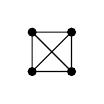
\begin{tikzpicture}[scale=0.5]
		\draw[fill] (0,0) circle [radius=0.1];
		\draw[fill] (0,1) circle [radius=0.1];
		\draw[fill] (1,0) circle [radius=0.1];
		\draw[fill] (1,1) circle [radius=0.1];
		
		\draw (0,0) -- (1, 0) -- (1, 0) -- (1, 1) -- (0, 1) -- (0, 0) -- (1, 1);
		\draw (1, 0) -- (0, 1);
		\end{tikzpicture} 
		&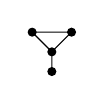
\begin{tikzpicture}[scale=0.5]
		\draw[fill] (0.5,0) circle [radius=0.1];
		\draw[fill] (0.5,0.5) circle [radius=0.1];
		\draw[fill] (0,1) circle [radius=0.1];
		\draw[fill] (1,1) circle [radius=0.1];
		
		\draw (0.5, 0) -- (0.5, 0.5) -- (1, 1) -- (0, 1) -- (0.5, 0.5);
		\end{tikzpicture}
		&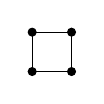
\begin{tikzpicture}[scale=0.5]
		\draw[fill] (0,0) circle [radius=0.1];
		\draw[fill] (0,1) circle [radius=0.1];
		\draw[fill] (1,0) circle [radius=0.1];
		\draw[fill] (1,1) circle [radius=0.1];
		
		\draw (0,0) -- (1, 0) -- (1, 1) -- (0, 1) -- (0, 0);
		\end{tikzpicture}  
		&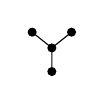
\begin{tikzpicture}[scale=0.5]
		\draw[fill] (0.5,0) circle [radius=0.1];
		\draw[fill] (0.5,0.6) circle [radius=0.1];
		\draw[fill] (0,1) circle [radius=0.1];
		\draw[fill] (1,1) circle [radius=0.1];
		
		\draw (0.5, 0) -- (0.5, 0.6) -- (1, 1);
		\draw (0.5, 0.6) -- (0, 1);
		\end{tikzpicture}    
		& 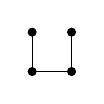
\begin{tikzpicture}[scale=0.5]
		\draw[fill] (0,0) circle [radius=0.1];
		\draw[fill] (0,1) circle [radius=0.1];
		\draw[fill] (1,0) circle [radius=0.1];
		\draw[fill] (1,1) circle [radius=0.1];
		
		\draw (0,1) -- (0, 0) -- (1, 0) -- (1, 1);
		\end{tikzpicture}   \\ \midrule
		CZ count & 14  & 14 & 16 & 16 & 18 \\
		CZ depth & 11  & 13 & 15 & 16 & 14 \\ \bottomrule       
	\end{tabular}
	\caption{Decompositions of 4q Toffoli gate on various topolgies}
	\label{tab toff4}
\end{table}

We now proceed to the decomposition of 4q Toffoli gates which are significantly more challenging. Variational synthesis of the 4q Toffoli gate on various 4q topologies has been recently addressed in \cite{Nakanishi2021}. Remarkably, the approach taken there was that of an exhaustive search over all architectures. It is interesting to note that for exhaustive search connectivity restrictions actually simplify the problem. Using \cpflow we were able to reproduce all results presented in \cite{Nakanishi2021}, see table \ref{tab toff4}. Moreover, for the star-shaped topology we achieved a minor improvement reducing the \CZ count from 17 to 16. The corresponding circuit is depicted at fig.\ref{fig toff4 star}. Note that we did not look for decompositions minimizing \CZ depth, but simply report \CZ depths of the first \CZ count optimal decompositions found during the search.

In all except for the fully connected topology, decompositions were discovered by the \adaptive algorithm with the full range of template depth for 4q unitaries (0, 61), 500 hundred samples at each hyperparameter configuration and 50 hyperparameter evaluations. The clock time taken by the search for each topology took about 40 minutes on our server \ref{server}. In contrast, the optimal decomposition on the fully connected topology only appeared after about 200 hyperparameter evaluations and took about 2 hours.

One might wonder why why did the exhaustive search approach of ref.\cite{Nakanishi2021} overlooked the 16 \CZ gates decomposition on the start topology? A possible cause might be found in the local minimums problem. Table tab.\ref{tab toff4 sr} shows empirical success ratios for optimal circuits found by \cpflow on the fully connected and star topologies. First thing to note is that the the success ratio for the star topology and XZ structure of 1q gates is only about $2\%$. Paper ref.\cite{Nakanishi2021} indeed used the XZ ansatz albeit with a different optimization procedure \cite{Nakanishi2020}. We find it likely that the appropriate architecture was missed simply due insufficient amount trials. The problem of local minimums in fact renders exhaustive search over the architectures insufficient to prove optimality of decompositions. Another interesting observation is that for a connected circuit the success rates of XYZ and XZ decompositions differ by an order of magnitude. This highlights the importance of the parametrization and/or initial sampling. 

\begin{table}[]
	\begin{tabular}{@{}cccccc@{}}
		\toprule
		 && XYZ && XZ &  \\ \midrule
		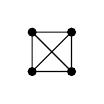
\begin{tikzpicture}[scale=0.5]
		\draw[fill] (0,0) circle [radius=0.1];
		\draw[fill] (0,1) circle [radius=0.1];
		\draw[fill] (1,0) circle [radius=0.1];
		\draw[fill] (1,1) circle [radius=0.1];
		
		\draw (0,0) -- (1, 0) -- (1, 0) -- (1, 1) -- (0, 1) -- (0, 0) -- (1, 1);
		\draw (1, 0) -- (0, 1);
		\end{tikzpicture}\quad  && $0.6\times10^{-2}$       && $7.8\times10^{-2}$ &  \\
		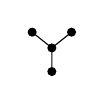
\begin{tikzpicture}[scale=0.5]
		\draw[fill] (0.5,0) circle [radius=0.1];
		\draw[fill] (0.5,0.6) circle [radius=0.1];
		\draw[fill] (0,1) circle [radius=0.1];
		\draw[fill] (1,1) circle [radius=0.1];
		
		\draw (0.5, 0) -- (0.5, 0.6) -- (1, 1);
		\draw (0.5, 0.6) -- (0, 1);
		\end{tikzpicture} \quad     && $0.4\times10^{-2}$     && $0.2\times10^{-2}$ 
		 &  \\ \bottomrule
	\end{tabular}
\caption {Empirical success ratios for optimal decompositions of the 4q Toffoli gate determined from 500 samples.}
\label{tab toff4 sr}
\end{table}




\begin{figure*}
\begin{align*}
\scalebox{0.65}{
	\Qcircuit @C=1.0em @R=0.2em @!R { \\
		& \gate{\mathrm{X}\,(\mathrm{\pi})} & \ctrl{1} & \gate{\mathrm{X}\,(\mathrm{\frac{\pi}{2}})} & \qw & \ctrl{2} & \gate{\mathrm{X}\,(\mathrm{\frac{\pi}{2}})} & \ctrl{3} & \ctrl{1} & \gate{\mathrm{Z}\,(\mathrm{\frac{-3\pi}{8}})} & \gate{\mathrm{X}\,(\mathrm{\frac{\pi}{2}})} & \ctrl{1} & \gate{\mathrm{Z}\,(\mathrm{\pi})} & \gate{\mathrm{X}\,(\mathrm{\frac{\pi}{2}})} & \ctrl{2} & \gate{\mathrm{X}\,(\mathrm{\frac{\pi}{2}})} & \ctrl{1} & \gate{\mathrm{X}\,(\mathrm{\frac{3\pi}{8}})} & \qw & \ctrl{3} & \gate{\mathrm{X}\,(\mathrm{\frac{7\pi}{8}})} & \ctrl{2} & \gate{\mathrm{Z}\,(\mathrm{\frac{-\pi}{2}})} & \gate{\mathrm{X}\,(\mathrm{\frac{\pi}{2}})} & \qw & \qw\\
		& \gate{\mathrm{X}\,(\mathrm{\frac{\pi}{2}})} & \control\qw & \gate{\mathrm{Z}\,(\mathrm{\frac{\pi}{2}})} & \gate{\mathrm{X}\,(\mathrm{\frac{\pi}{8}})} & \qw & \qw & \qw & \control\qw & \gate{\mathrm{Z}\,(\mathrm{\pi})} & \gate{\mathrm{X}\,(\mathrm{\frac{5\pi}{8}})} & \control\qw & \gate{\mathrm{X}\,(\mathrm{\frac{\pi}{2}})} & \qw & \qw & \qw & \control\qw & \gate{\mathrm{Z}\,(\mathrm{\frac{-\pi}{2}})} & \gate{\mathrm{X}\,(\mathrm{\frac{\pi}{2}})} & \qw & \qw & \qw & \qw & \qw & \qw & \qw\\
		& \gate{\mathrm{X}\,(\mathrm{\pi})} & \qw & \qw & \qw & \control\qw & \gate{\mathrm{X}\,(\mathrm{\pi})} & \qw & \qw & \qw & \qw & \qw & \qw & \qw & \control\qw & \gate{\mathrm{X}\,(\mathrm{\pi})} & \qw & \qw & \qw & \qw & \qw & \control\qw & \qw & \qw & \qw & \qw\\
		& \qw & \qw & \qw & \qw & \qw & \qw & \control\qw & \gate{\mathrm{Z}\,(\mathrm{\frac{\pi}{2}})} & \gate{\mathrm{X}\,(\mathrm{\frac{\pi}{2}})} & \qw & \qw & \qw & \qw & \qw & \qw & \qw & \qw & \qw & \control\qw & \gate{\mathrm{Z}\,(\mathrm{\frac{-5\pi}{8}})} & \gate{\mathrm{X}\,(\mathrm{\frac{\pi}{2}})} & \qw & \qw & \qw & \qw\\
		\\ }}
\\
\scalebox{0.65}{
	\Qcircuit @C=1.0em @R=0.2em @!R { \\
		& \ctrl{3} & \gate{\mathrm{Z}\,(\mathrm{\frac{\pi}{8}})} & \gate{\mathrm{X}\,(\mathrm{\frac{\pi}{2}})} & \ctrl{1} & \gate{\mathrm{Z}\,(\mathrm{\frac{-\pi}{2}})} & \gate{\mathrm{X}\,(\mathrm{\frac{3\pi}{8}})} & \ctrl{3} & \gate{\mathrm{Z}\,(\mathrm{-\pi})} & \gate{\mathrm{X}\,(\mathrm{\frac{\pi}{8}})} & \ctrl{2} & \gate{\mathrm{Z}\,(\mathrm{\frac{-\pi}{2}})} & \gate{\mathrm{X}\,(\mathrm{\frac{\pi}{2}})} & \ctrl{3} & \gate{\mathrm{Z}\,(\mathrm{\frac{7\pi}{8}})} & \gate{\mathrm{X}\,(\mathrm{\frac{\pi}{2}})} & \ctrl{1} & \gate{\mathrm{Z}\,(\mathrm{\frac{-\pi}{2}})} & \gate{\mathrm{X}\,(\mathrm{\frac{5\pi}{8}})} & \ctrl{3} & \gate{\mathrm{Z}\,(\mathrm{\frac{-\pi}{2}})} & \gate{\mathrm{X}\,(\mathrm{\frac{\pi}{2}})} & \gate{\mathrm{Z}\,(\mathrm{\frac{-3\pi}{8}})} & \qw & \qw\\
		& \qw & \qw & \qw & \control\qw & \qw & \qw & \qw & \qw & \qw & \qw & \qw & \qw & \qw & \qw & \qw & \control\qw & \gate{\mathrm{X}\,(\mathrm{\pi})} & \gate{\mathrm{Z}\,(\mathrm{\frac{-7\pi}{8}})} & \qw & \qw & \qw & \qw & \qw & \qw\\
		& \qw & \qw & \qw & \qw & \qw & \qw & \qw & \qw & \qw & \control\qw & \gate{\mathrm{X}\,(\mathrm{\pi})} & \gate{\mathrm{Z}\,(\mathrm{\frac{-3\pi}{8}})} & \qw & \qw & \qw & \qw & \qw & \qw & \qw & \qw & \qw & \qw & \qw & \qw\\
		& \control\qw & \gate{\mathrm{X}\,(\mathrm{\frac{\pi}{2}})} & \qw & \qw & \qw & \qw & \control\qw & \gate{\mathrm{Z}\,(\mathrm{\frac{\pi}{2}})} & \gate{\mathrm{X}\,(\mathrm{\frac{\pi}{2}})} & \qw & \qw & \qw & \control\qw & \gate{\mathrm{X}\,(\mathrm{\frac{\pi}{2}})} & \qw & \qw & \qw & \qw & \control\qw & \gate{\mathrm{Z}\,(\mathrm{\frac{-3\pi}{8}})} & \gate{\mathrm{X}\,(\mathrm{\frac{\pi}{2}})} & \gate{\mathrm{Z}\,(\mathrm{\frac{\pi}{2}})} & \qw & \qw\\
		\\ }}
\end{align*}	
\caption{Decomposition of the 4q Toffoli gate on the star topology with 16 \CZ-gates}
\label{fig toff4 star}
\end{figure*}
\subsection{Toffoli 5}
To our knowledge, the best decomposition of the 5q Toffoli gate on a fully connected topology without ancilla qubits features $30$ \CZ gates, an upper bound valid for all diagonal gates \cite{Shende2006}. The best result of direct synthesis with \cpflow running for several hours that we observed featured 36 \CZ gates indicating that 5q unitaries are significantly harder to address. However, synthesis with topological restrictions also poses significant challenges to the mulpilexing decomposition framework of \cite{Shende2006}. It is thus still interesting to see if our numerical routine can be useful. 

To this end we consider compilation of 5q Toffoli gate on the chain topology. As a reference point we take the best compilation out of 1000 runs of the qiskit transpiler with \param{optimization\_level} set to 3 that yields a 61 \CZ count decomposition \footnote{Note that the transpillation process in qiskit genrally yields circuits which only equal to the target unitaries up to possible permutations of qubits. As restoring the original permutation might be an expensive operation in terms of the \CZ count the transpilation results should really be considered as a lower bound.}. The best results of direct synthesis with \cpflow yielded a decomposition with 69 \CZ gates. As we now show, by using a combination of the analytic and numerical techniques this this result can be improved to 48 \CZ gates. 

Our strategy is to reduce compilation into several 4q blocks. We first observe that the optimal 30 \CZ gate decomposition of the 5q Toffoli gate on a fully connected topology can be obtained from the left circuit depicted at fig.\eqref{fig toff5}. Triply controlled $\sqrt{\text{X}}$ gate is a diagonal gate up to conjugation by the Hadamard gates and hence can be decomposed into 14 \CZ gates, just as the standard 4q Toffoli gate. Singly controlled $\sqrt{\text{X}}$ can be decomposed into 2 \CZ gates each. Finally the boxed 4q Toffoli gates can be replaced by their relative phase counterparts \cite{Maslov} which have \CZ count just 6. In total this gives 30 \CZ gates, the optimal amount. 

We now try to adapt this decomposition to the chain topology. Right circuit on fig.\ref{fig toff5} shows that by inserting four additional $\CX$ gates (each pair originates from a SWAP gate, the two closest $\CX$ gates cancel each other) around triply controlled $\sqrt{\text{X}}$ we can place all 4q gates on the first four qubits. Next, we use \cpflow to decompose $\sqrt{\text{X}}$ and relative phase \cx{3} gates on a chain topology. We found a 18 \CZ decomposition of the C${}^{3}\sqrt{\text{X}}$, the same gate count that is needed for decomposition of the \cx{3} gate on a chain topology \ref{tab toff4}. For the relative phase \cx{3} gates we found 11 \CZ decompositions. This yields the decomposition of the 5q Toffoli gate on the chain topology with $48=2\times 11+18+2\times4$ \CZ gates in total. We are not aware of other existing methods could improve on this count.

\begin{figure*}
	\begin{align}
	\Qcircuit @C=1.0em @R=0.2em @!R {
		\qquad& \ctrl{1} & \qw & \ctrl{1} & \qw & \ctrl{1} & \qw & \qw\\
		\qquad& \ctrl{1} & \qw & \ctrl{1} & \qw & \ctrl{1} & \qw & \qw\\
		C^{4}X=\qquad\qquad& \ctrl{1} & \qw & \ctrl{1} & \qw & \ctrl{2} & \qw & \qw\\
		\qquad& \targ & \ctrl{1} & \targ & \ctrl{1} & \qw & \qw & \qw\\
		\qquad& \qw & \gate{\mathrm{\sqrt{X}^\dagger}} & \qw & \gate{\mathrm{\sqrt{X}}} & \gate{\mathrm{\sqrt{X}}} & \qw & \qw \gategroup{1}{2}{4}{2}{1em}{--}
		\gategroup{1}{4}{4}{4}{1em}{--}
	}\raisebox{-4em}{\qquad=\qquad}
	\Qcircuit @C=1.0em @R=0.2em @!R {
		& \ctrl{1} & \qw & \ctrl{1} & \qw & \qw & \qw & \ctrl{1} & \qw & \qw & \qw & \qw\\
		& \ctrl{1} & \qw & \ctrl{1} & \qw & \qw & \qw & \ctrl{1} & \qw & \qw & \qw & \qw\\
		& \ctrl{1} & \qw & \ctrl{1} & \qw & \qw & \qw & \ctrl{1} & \qw & \qw & \qw & \qw\\
		& \targ & \ctrl{1} & \targ & \ctrl{1} & \targ & \ctrl{1} & \gate{\mathrm{\sqrt{X}}} & \ctrl{1} & \targ & \qw & \qw\\
		& \qw & \gate{\mathrm{\sqrt{X}^\dagger}} & \qw & \gate{\mathrm{\sqrt{X}}} & \ctrl{-1} & \targ & \qw & \targ & \ctrl{-1} & \qw & \qw 
		\gategroup{1}{2}{4}{2}{1em}{--}
		\gategroup{1}{4}{4}{4}{1em}{--}
	}
	\end{align}	 
	\caption{A decomposition of the 5q Toffoli gate.}
	\label{fig toff5}
\end{figure*}

\section{Further benchmarks \label{sec benchmark}}
\begin{table*}[]
	\begin{tabular}{@{}ccccc@{}}
		\toprule\toprule
		Circuit               & CPFlow \qquad & SQUANDER \qquad & QSearch \qquad & QFast+Qiskit+SQUANDER \qquad \\ \midrule\midrule
		\multicolumn{5}{c}{Connected, lower complexity}                              \\ \midrule
		4gt5\_76              & 21      & 24       & -       & -                     \\
		one-two-three-v2\_100 & 28      & 37       & 43      & -                     \\
		alu-v3\_34            & 14      & 25       & 27      & -                     \\
		alu-v4\_36            & 30      & 40       & -       & -                     \\
		4gt13\_92             & 17      & 24       & -       & -                     \\ \midrule
		\multicolumn{5}{c}{Chain, lower complexity}                                  \\ \midrule
		4gt13\_91             & 26(/30) & 26       & 35      & -                     \\
		4gt5\_76              & -1      & 26       & 51      & -                     \\
		alu-v0\_26            & 28      & 32       & -       & -                     \\
		alu-v3\_35            & 24      & 26       & 34      & -                     \\
		4mod5-v1\_24          & 29      & 31       & 44      & -                     \\ \midrule
		\multicolumn{5}{c}{Connected, higher complexity}                             \\ \midrule
		4gt10-v1\_81          & 39(/36) & -        & -       & 39                    \\
		one-two-three-v1\_99  & -1      & -        & -       & 45                    \\
		one-two-three-v0\_98  & -1      & -        & -       & 61                    \\
		aj-e11\_165           & 24      & -        & -       & 36                    \\
		alu-v2\_32            & 30      & -        & -       & 41                   
	\end{tabular}
\end{table*}

Following \cite{Rakyta2022} we test the performance of \package{CPFlow} on a range of standard benchmark circuits from the ibm\_qx database \cite{Zulehner2019, ibm_qx}. In \cite{Rakyta2022} an extensive comparison between packages \package{SQUANDER}, \package{QFast}, \package{QSearch} was performed. The \package{SQUANDER} reliably outperformed other packages in almost every single example. From each of the tables 1, 3 and 4 presented in \cite{Rakyta2022} we pick 5 circuits with the highest \CZ count found by \package{SQUANDER}, as these are likely to be the most challenging and hence the most informative (for the same reason we skipped table 2, which mostly contains much simpler circuits). All selected examples are 5q circuits. We processed these circuits with \cpflow, results are reported in tab.\ref{tab bench}.

Results for the connected circuits of the lower complexity show a significant compression averaging to approximately 25\% compared to the \package{SQUANDER} results. In contrast, for circuits of similar complexity on the chain topology the difference between \package{CPFlow} and \package{SQUANDER} is less noticeable, averaging to $xx$\%. It would be interesting to understand the role of topology in either approach in more detail. Finally, circuits of greater complexity on a connected topology...


\section{Summary and outlook \label{sec last}}
In this paper we presented a new approach to the variational synthesis into CNOT/\CZ+1q gate set. We identified the problem of local minimums as a crucial yet underappreciated obstacle that needs to be addressed. In the absence of an efficient way to avoid local minimums we have made an extensive exploration of the initial conditions space an integral part of our approach. We also proposed to use parametric 2q gates as a way to unify the architecture search with the continuous optimization of 1q gates into a single coherent optimization and demonstrated its efficiency. A recent work based on a similar idea \cite{Rakyta2022} also showed significant improvement over more standard discrete architecture search \cite{Smith2021}.

While capable to generate many interesting results our approach has its limitations. The first is rather fundamental and common to all similar schemes. Since the input circuit is represented by means of the corresponding unitary matrix, only small scale circuits that are easy to simulate classically can be addressed. This however does not preclude using variational synthesis to optimize smaller building blocks of large scale useful quantum algorithms \cite{Younis2021}. Exploring this direction is an important and practically relevant avenue for future work.

Scaling up the variational approach within the classically accessible regime appears to be mostly limited by the circuit complexity rather than the qubit count, e.g. it seems to be more difficult to efficiently compile a 4q circuit that requires many 2q gates than it is to compile a 5q circuit that can be represented using only a small amount of 2q gates. Importantly, the challenges associated with the higher complexity are not caused only by the combinatorial growth of the possible architectures but also by the proliferation of the local minimums in the loss landscape. Our empirical results (cf fig.\ref{fig local minumums}) indicate that already for 4q circuits in the range from 12 to 50 2q gates the probability of successful continuous optimization is less than 0.1\% even for a correctly chosen architecture. This probability depends on numerous factors including details of the optimization procedure, distribution of the initial conditions and parametrization of the loss landscape. Detailed understanding of these mechanisms may lead to a dramatic improvement in variational compilers efficiency.

There is also another interesting possibility to enhance variational synthesis of high-complexity unitaries. If the unitary originates from a known quantum circuit, it could be possible to use this information to ones advantage. For example, splitting the original circuit in parts each having lower complexity and synthesising them separately may lead to better results. Another proposal is to use the original circuit as the starting template for the variational compression \cite{Rakyta2022}. Eventually, the viability and resource allowance of the variational synthesis must be justified by the payoff if provides for useful applications.


\subsection*{Acknowledgments}

\appendix
\section{Gates}

\section{Circuit refinement}
Quantum circuits that result from numerical optimization performed by \cpflow typically have many redundant 1q gates, see fig.\ref{fig ref circuit}(a) for an example. As a function of a single angle any parametrized quantum circuit with rotation gates has the following simple form
\begin{align}
U(a)=U_0 \cos a+U_1\sin a
\end{align}
with some unitary matrices $U_0, U_1$. In turn, as a function of two angles it can always be represented as
\begin{align}
U(a_1, a_2)=U_{00}\cos a_1\cos a_2+U_{01}\cos a_1\sin a_2+U_{10}\sin a_1\cos a_2+U_{11}\sin a_1 a_2 = W_0 \cos(a_1+a_2)+W_1 \cos(a_1-a_2)+W_2\sin (a_1+a_2)+W_3\cos(a_1-a_2)
\end{align}
Typically all the terms in the rhs are non-vanishing and different choices of $a_1, a_2$ correspond to different unitaries (up to discrete redundancies). It may happen, however

\begin{figure*}
\begin{flushleft}
(a) Original circuit
	\begin{multline*}
	\Qcircuit @C=1.0em @R=0.2em @!R { \\
		& \gate{\mathrm{Z}\,(\mathrm{\frac{\pi}{2}})} & \gate{\mathrm{X}\,(\mathrm{\pi})} & \gate{\mathrm{Z}\,(\mathrm{0})} & \ctrl{1} & \gate{\mathrm{Z}\,(\mathrm{-2.356})} & \gate{\mathrm{X}\,(\mathrm{1.257e-05})} & \gate{\mathrm{Z}\,(\mathrm{4.511})} & \qw & \qw\\
		& \gate{\mathrm{Z}\,(\mathrm{0})} & \gate{\mathrm{X}\,(\mathrm{0.7854})} & \gate{\mathrm{Z}\,(\mathrm{\frac{\pi}{2}})} & \control\qw & \gate{\mathrm{Z}\,(\mathrm{-3.142})} & \gate{\mathrm{X}\,(\mathrm{1.571})} & \gate{\mathrm{Z}\,(\mathrm{3.685})} & \qw & \qw\\
		& \gate{\mathrm{Z}\,(\mathrm{0})} & \gate{\mathrm{X}\,(\mathrm{1.489})} & \gate{\mathrm{Z}\,(\mathrm{3.142})} & \qw & \qw & \qw & \qw & \qw & \qw}\\
	\Qcircuit @C=1.0em @R=0.2em @!R { \\
		& \gate{\mathrm{Z}\,(\mathrm{\frac{\pi}{2}})} & \gate{\mathrm{X}\,(\mathrm{\pi})} & \gate{\mathrm{Z}\,(\mathrm{0})} & \ctrl{1} & \gate{\mathrm{Z}\,(\mathrm{-2.356})} & \gate{\mathrm{X}\,(\mathrm{1.257e-05})} & \gate{\mathrm{Z}\,(\mathrm{4.511})} & \qw & \qw\\
		& \gate{\mathrm{Z}\,(\mathrm{0})} & \gate{\mathrm{X}\,(\mathrm{0.7854})} & \gate{\mathrm{Z}\,(\mathrm{\frac{\pi}{2}})} & \control\qw & \gate{\mathrm{Z}\,(\mathrm{-3.142})} & \gate{\mathrm{X}\,(\mathrm{1.571})} & \gate{\mathrm{Z}\,(\mathrm{3.685})} & \qw & \qw\\
		& \gate{\mathrm{Z}\,(\mathrm{0})} & \gate{\mathrm{X}\,(\mathrm{1.489})} & \gate{\mathrm{Z}\,(\mathrm{3.142})} & \qw & \qw & \qw & \qw & \qw & \qw}
	\end{multline*}
	
(b) Circuit with reduced angles.

	\scalebox{0.6}{
		\Qcircuit @C=1.0em @R=0.2em @!R { \\
			& \gate{\mathrm{X}\,(\mathrm{3.142})} & \ctrl{2} & \qw & \qw & \qw & \qw & \qw & \ctrl{2} & \qw & \qw & \qw & \qw & \ctrl{1} & \gate{\mathrm{X}\,(\mathrm{-\pi})} & \qw & \ctrl{1} & \gate{\mathrm{Z}\,(\mathrm{0.7852})} & \qw & \qw & \qw & \qw\\
			& \qw & \qw & \qw & \qw & \ctrl{1} & \gate{\mathrm{X}\,(\mathrm{3.141})} & \qw & \qw & \qw & \qw & \ctrl{1} & \gate{\mathrm{X}\,(\mathrm{1.571})} & \control\qw & \gate{\mathrm{Z}\,(\mathrm{-1.571})} & \gate{\mathrm{X}\,(\mathrm{0.7854})} & \control\qw & \gate{\mathrm{Z}\,(\mathrm{-1.571})} & \gate{\mathrm{X}\,(\mathrm{1.571})} & \gate{\mathrm{Z}\,(\mathrm{-2.357})} & \qw & \qw\\
			& \qw & \control\qw & \gate{\mathrm{Z}\,(\mathrm{-\pi})} & \gate{\mathrm{X}\,(\mathrm{2.356})} & \control\qw & \gate{\mathrm{Z}\,(\mathrm{-\pi})} & \gate{\mathrm{X}\,(\mathrm{2.356})} & \control\qw & \gate{\mathrm{Z}\,(\mathrm{-\pi})} & \gate{\mathrm{X}\,(\mathrm{0.7853})} & \control\qw & \gate{\mathrm{Z}\,(\mathrm{-3.142})} & \gate{\mathrm{X}\,(\mathrm{-0.7855})} & \gate{\mathrm{Z}\,(\mathrm{3.142})} & \qw & \qw & \qw & \qw & \qw & \qw & \qw}}
\vspace{2em}

(c) Rationalized circuit.
	
	\scalebox{0.7}{
		\Qcircuit @C=1.0em @R=0.2em @!R { \\
			& \gate{\mathrm{X}\,(\mathrm{\pi})} & \ctrl{2} & \qw & \qw & \qw & \qw & \qw & \ctrl{2} & \qw & \qw & \qw & \qw & \ctrl{1} & \gate{\mathrm{X}\,(\mathrm{-\pi})} & \qw & \ctrl{1} & \gate{\mathrm{Z}\,(\mathrm{\frac{\pi}{4}})} & \qw & \qw & \qw & \qw\\
			& \qw & \qw & \qw & \qw & \ctrl{1} & \gate{\mathrm{X}\,(\mathrm{\pi})} & \qw & \qw & \qw & \qw & \ctrl{1} & \gate{\mathrm{X}\,(\mathrm{\frac{\pi}{2}})} & \control\qw & \gate{\mathrm{Z}\,(\mathrm{\frac{-\pi}{2}})} & \gate{\mathrm{X}\,(\mathrm{\frac{\pi}{4}})} & \control\qw & \gate{\mathrm{Z}\,(\mathrm{\frac{-\pi}{2}})} & \gate{\mathrm{X}\,(\mathrm{\frac{\pi}{2}})} & \gate{\mathrm{Z}\,(\mathrm{\frac{-3\pi}{4}})} & \qw & \qw\\
			& \qw & \control\qw & \gate{\mathrm{Z}\,(\mathrm{-\pi})} & \gate{\mathrm{X}\,(\mathrm{\frac{3\pi}{4}})} & \control\qw & \gate{\mathrm{Z}\,(\mathrm{-\pi})} & \gate{\mathrm{X}\,(\mathrm{\frac{3\pi}{4}})} & \control\qw & \gate{\mathrm{Z}\,(\mathrm{-\pi})} & \gate{\mathrm{X}\,(\mathrm{\frac{\pi}{4}})} & \control\qw & \gate{\mathrm{Z}\,(\mathrm{-\pi})} & \gate{\mathrm{X}\,(\mathrm{\frac{-\pi}{4}})} & \gate{\mathrm{Z}\,(\mathrm{\pi})} & \qw & \qw & \qw & \qw & \qw & \qw & \qw}}
\end{flushleft}		
\caption{Circuit refinement}
\label{fig ref circuit}
\end{figure*}

\bibliographystyle{/home/idnm/Dropbox/hep/Sheets/utcaps_edited}
\bibliography{/home/idnm/Dropbox/hep/Sheets/library.bib, bibfile.bib}
\end{document}
